% https://es.overleaf.com/latex/templates/project-report/jpzczmpsdzwm

%%% Preamble
\documentclass[paper=leter, fontsize=11pt]{scrartcl}
\usepackage[utf8]{inputenc}
\usepackage[spanish,mexico]{babel}
\usepackage[T1]{fontenc}    % use 8-bit T1 fonts
\usepackage{lmodern}
\usepackage{hyperref}       % hyperlinks
\usepackage{lipsum}
\usepackage[square,numbers]{natbib}

\usepackage[protrusion=true,expansion=true]{microtype}	
\usepackage{amsmath,amsfonts,amsthm} % Math packages
\usepackage[pdftex]{graphicx}
\usepackage{url}
 
\usepackage{booktabs}
\usepackage[table,xcdraw]{xcolor}

\usepackage{tikz}
\usetikzlibrary{positioning,matrix, arrows.meta}

\usepackage{caption} 
\usepackage{subcaption}


\usepackage{listings}
\lstdefinestyle{mystyle}{ 
    basicstyle=\ttfamily\footnotesize,
    breakatwhitespace=false,         
    breaklines=true,                 
    captionpos=b,                    
    keepspaces=true,                 
    numbers=left,                    
    numbersep=5pt,                  
    showspaces=false,                
    showstringspaces=false,
    showtabs=false,                  
    tabsize=4
}

\lstset{style=mystyle}
\renewcommand{\lstlistingname}{Código}


\selectlanguage{spanish}
\usepackage[spanish,onelanguage,ruled]{algorithm2e}


%%% Custom sectioning
\usepackage{sectsty}
\allsectionsfont{\centering \normalfont\scshape}


%%% Custom headers/footers (fancyhdr package)
\usepackage{fancyhdr}
\pagestyle{fancyplain}
\fancyhead{}											% No page header
\fancyfoot[L]{}											% Empty 
\fancyfoot[C]{}											% Empty
\fancyfoot[R]{\thepage}									% Pagenumbering
\renewcommand{\headrulewidth}{0pt}			% Remove header underlines
\renewcommand{\footrulewidth}{0pt}				% Remove footer underlines
\setlength{\headheight}{13.6pt}


%%% Equation and float numbering
\numberwithin{equation}{section}		% Equationnumbering: section.eq#
\numberwithin{figure}{section}			% Figurenumbering: section.fig#
\numberwithin{table}{section}				% Tablenumbering: section.tab#


%%% Maketitle metadata
\newcommand{\horrule}[1]{\rule{\linewidth}{#1}} 	% Horizontal rule

%%% https://tex.stackexchange.com/a/118217
\usepackage{mathtools}
\DeclarePairedDelimiter\ceil{\lceil}{\rceil}
\DeclarePairedDelimiter\floor{\lfloor}{\rfloor}

\usepackage{amsmath}

\usepackage{tikz}

\title{
		%\vspace{-1in} 	
		\usefont{OT1}{bch}{b}{n}
		\normalfont \normalsize \textsc{Posgrado de Ingeniería de Sistemas} \\ [25pt]
		\horrule{0.5pt} \\[0.4cm]
		\huge Distribuciones en oraciones de Dracula \\
		\horrule{2pt} \\[0.5cm]
}
\author{
		\normalfont 								\normalsize
        Alberto Benavides\\[-3pt]		\normalsize
        \today
}
\date{}


%%% Begin document
\begin{document}
\maketitle

\section{Introducción}

En este trabajo me apoyé con Gabriela Sánchez Yépez con repositorio ubicado en \url{https://github.com/Saphira3000/MPA} para realizar las distribuciones binomial negativa y geométrica del final.

Existen diversos métodos para determinar la autoría de libros. De entre ellos destaca el que utiliza minería de textos combinado con técnicas de agrupamientos como $K$--medias. Estos métodos utilizan como sus características la cantidad de palabras y comas de las oraciones presentes en las obras, entre otras. Un breve ejemplo sobre esta técnica se halla en \url{http://www.aicbt.com/authorship-attribution/}.

\section{Recursos}

El libro de \textit{Dracula} \cite{dracula1897} escrito por \citeauthor*{dracula1897} en \citeyear{dracula1897} se encuentra disponible de manera gratuita en el sitio de Project Gutenberg \cite{dracula}. Éste se descarga por la librería \texttt{gutembergr} \cite{gutenbergr} de R. La separación en oraciones se realiza mediante \texttt{corpus} \cite{corpus}.

\section{Preprocesamiento}
Después de obtenido el libro mediante la función \texttt{gutenberg\_download}, se analiza su contenido inicial y final con las funciones \texttt{head} y \texttt{tail}. Esto muestra la existencia de apartados introductorios y anexos que se escapan del contenido del libro en sí, por lo que se procede a remover del contenido esos elementos. Destaca aquí el uso de la función \texttt{grep} que permite identificar expresiones regulares y, en este caso, la ubicación del final del libro que coindice con las palabras ``THE END''.

\section{Resultados y análisis}
Con el contenido del libro se pueden extraer las oraciones que contiene. Para ello primero es necesario convertir el libro obtenido en una sola cadena de texto, lo que se hace con la función \texttt{paste}, seguido del uso de la función \texttt{text\_split} de la librería \texttt{corpus} que separa las oraciones de dicho texto. Se prefiere el uso de esta librería puesto que obvia abreviaturas que usan puntos para evitar separar oraciones por estos motivos. De estas oraciones se cuentan las palabras que contienen y las comas con \texttt{strsplit} para la primera y \texttt{str\_count} para la última. Enseguida se grafican los histogramas de palabras y comas por oración junto a una función de distribución que se equipara a sus proporciones. Estas gráficas pueden verse en las figuras \ref{palabras} (p. \pageref{palabras}) y \ref{comas} (p. \pageref{comas}), respectivamente. Los procedimientos computacionales y sus códigos pueden revisarse en \url{https://github.com/jbenavidesv87/probabilidad/blob/master/tema3/tarea.ipynb}

\begin{figure}
    \centering
    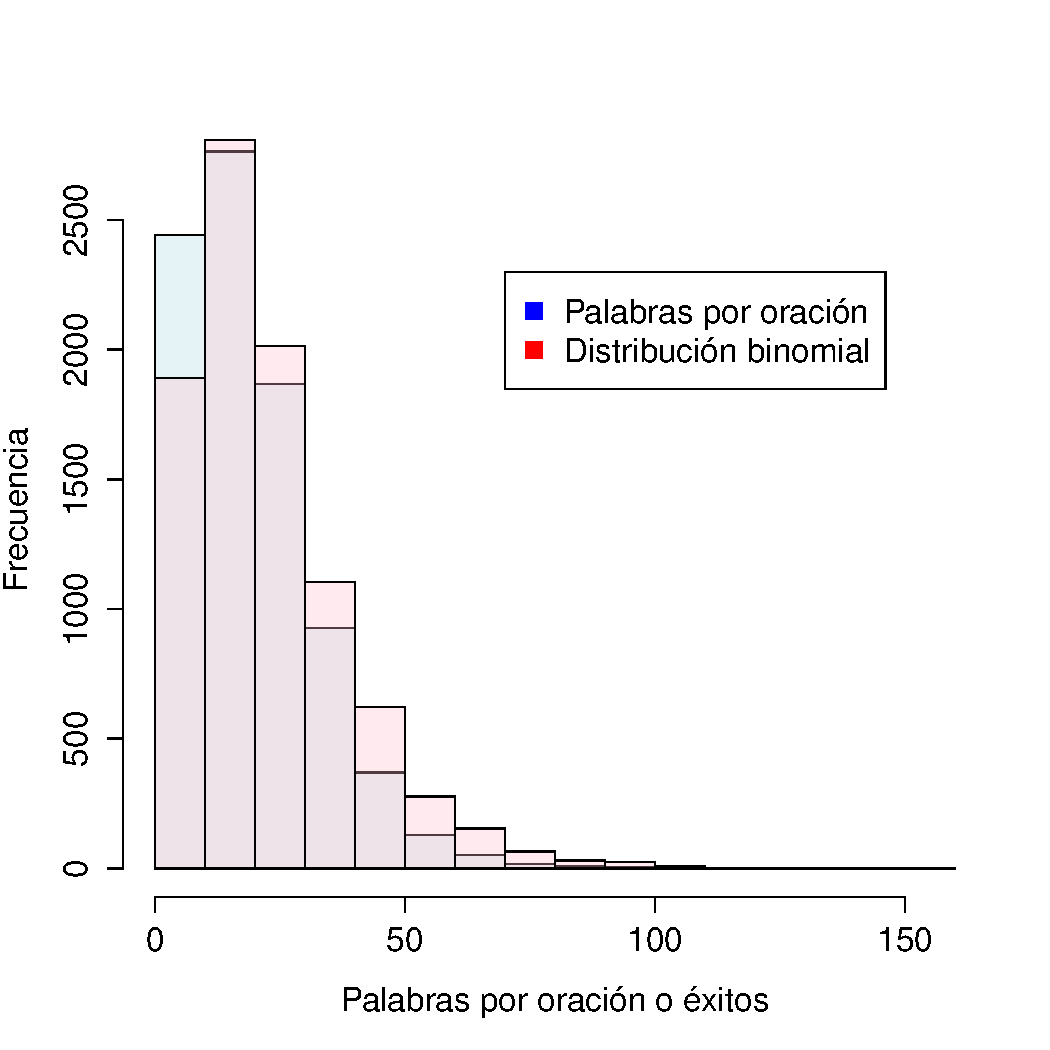
\includegraphics[width=1\textwidth]{palabras.pdf}
    \caption{Histogramas de palabras por oración de \textit{Dracula} (azul) y función de distribución binomial negativa (rojo).}
    \label{palabras}
\end{figure}

\begin{figure}
    \centering
    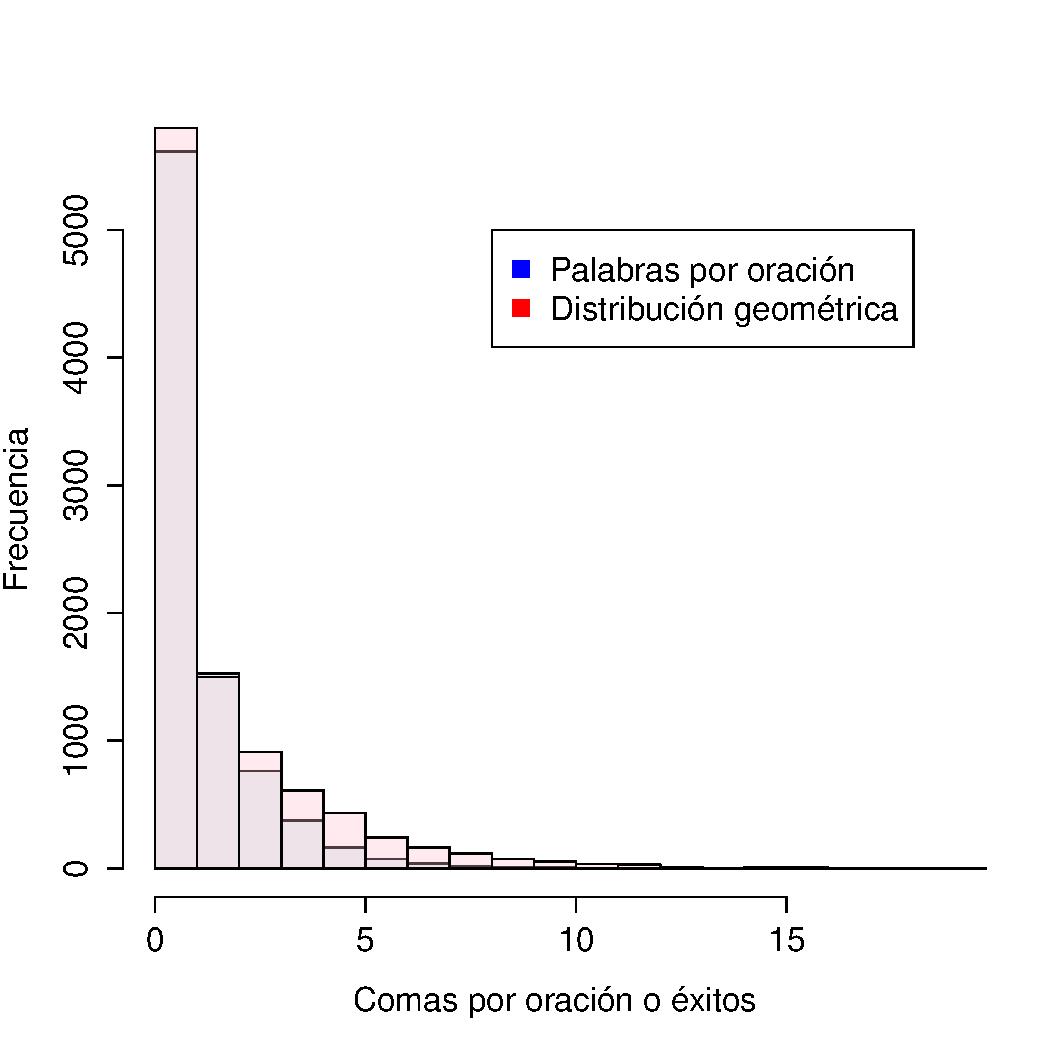
\includegraphics[width=1\textwidth]{comas.pdf}
    \caption{Histogramas de comas por oración de \textit{Dracula} (azul) y función de distribución geométrica (rojo).}
    \label{comas}
\end{figure}

La distribución de palabras por oración que sigue la obra de \textit{Dracula} coincide con una distribución binomial negativa. Este tipo de distribuciones se generan tras obtener, en un transcurso de $r_1$ repeticiones, las veces que debe repetirse un experimento para que un determinado evento con probabilidad $p_1$ sea exitoso un total de $k$ veces. En este caso, la distribución binomial negativa generada que equipara los resultados de la distribución del número de palabras por oración, toma los parámetros $r_1 = 90000$, $p_1 = 0.087$ y $k = 2$.

Por su parte, la distribución de comas en una oración de la obra citada coincide con una distribución geométrica que se desarrolla a partir del número de veces que debe hacerse un experimento de probabilidad $p_2$ (repetido $r_2$ veces) para que tal experimento sea exitoso una primera vez. Los parámetros que toma esta distribución para ser semejante a la del número de comas por oración en \textit{Dracula} son $p_2 = 0.35$ y $r_2 = 10000$.

\bibliographystyle{plainnat}
\bibliography{Biblio}

\end{document}